\section{Wyniki własne}

\begin{frame}{Środowiska testowe}
\textbf{Wykorzystane modele do weryfikacji algorytmów:}

\begin{enumerate}
    \item \textbf{MDP z dwoma stanami}
    \begin{itemize}
        \item Prosty model do weryfikacji analitycznej
        \item 2 stany, 2 akcje
        \item Możliwość dokładnego obliczenia wartości optymalnych
    \end{itemize}
    
    \vspace{0.5em}
    \item \textbf{Problem zarządzania zapasami}
    \begin{itemize}
        \item Bardziej złożone środowisko
        \item Modelowanie rzeczywistych decyzji biznesowych
        \item Testowanie w warunkach zbliżonych do praktycznych zastosowań
    \end{itemize}
\end{enumerate}

\vspace{0.5em}
\textbf{Parametry eksperymentów:}
\begin{itemize}
    \item Współczynnik uprzedzenia teraźniejszości: $\alpha = 0.5$
    \item Współczynnik dyskontowania: $\beta = 0.9$
    \item Polityka próbkowania: uniform (eksploracja całej przestrzeni)
\end{itemize}
\end{frame}

\begin{frame}{MDP z dwoma stanami -- Model}
\begin{columns}
\begin{column}{0.5\textwidth}
\textbf{Definicja modelu:}
\begin{itemize}
    \item Stany: $S = \{1, 2\}$
    \item Akcje: $A = \{a_1, a_2\}$
    \item Parametry: $\alpha = 0.5$, $\beta = 0.9$
\end{itemize}

\vspace{0.5em}
\textbf{Nagrody:}
\begin{itemize}
    \item $r(1,a_1) = 0$
    \item $r(1,a_2) = 2$
    \item $r(2,a_1) = 15$
    \item $r(2,a_2) = 20$ lub $5$
\end{itemize}

\vspace{0.5em}
\textbf{Testowane polityki:}
\begin{itemize}
    \item 4 deterministyczne
    \item 1 mieszana (50/50)
\end{itemize}
\end{column}

\begin{column}{0.5\textwidth}
\begin{figure}
    \centering
    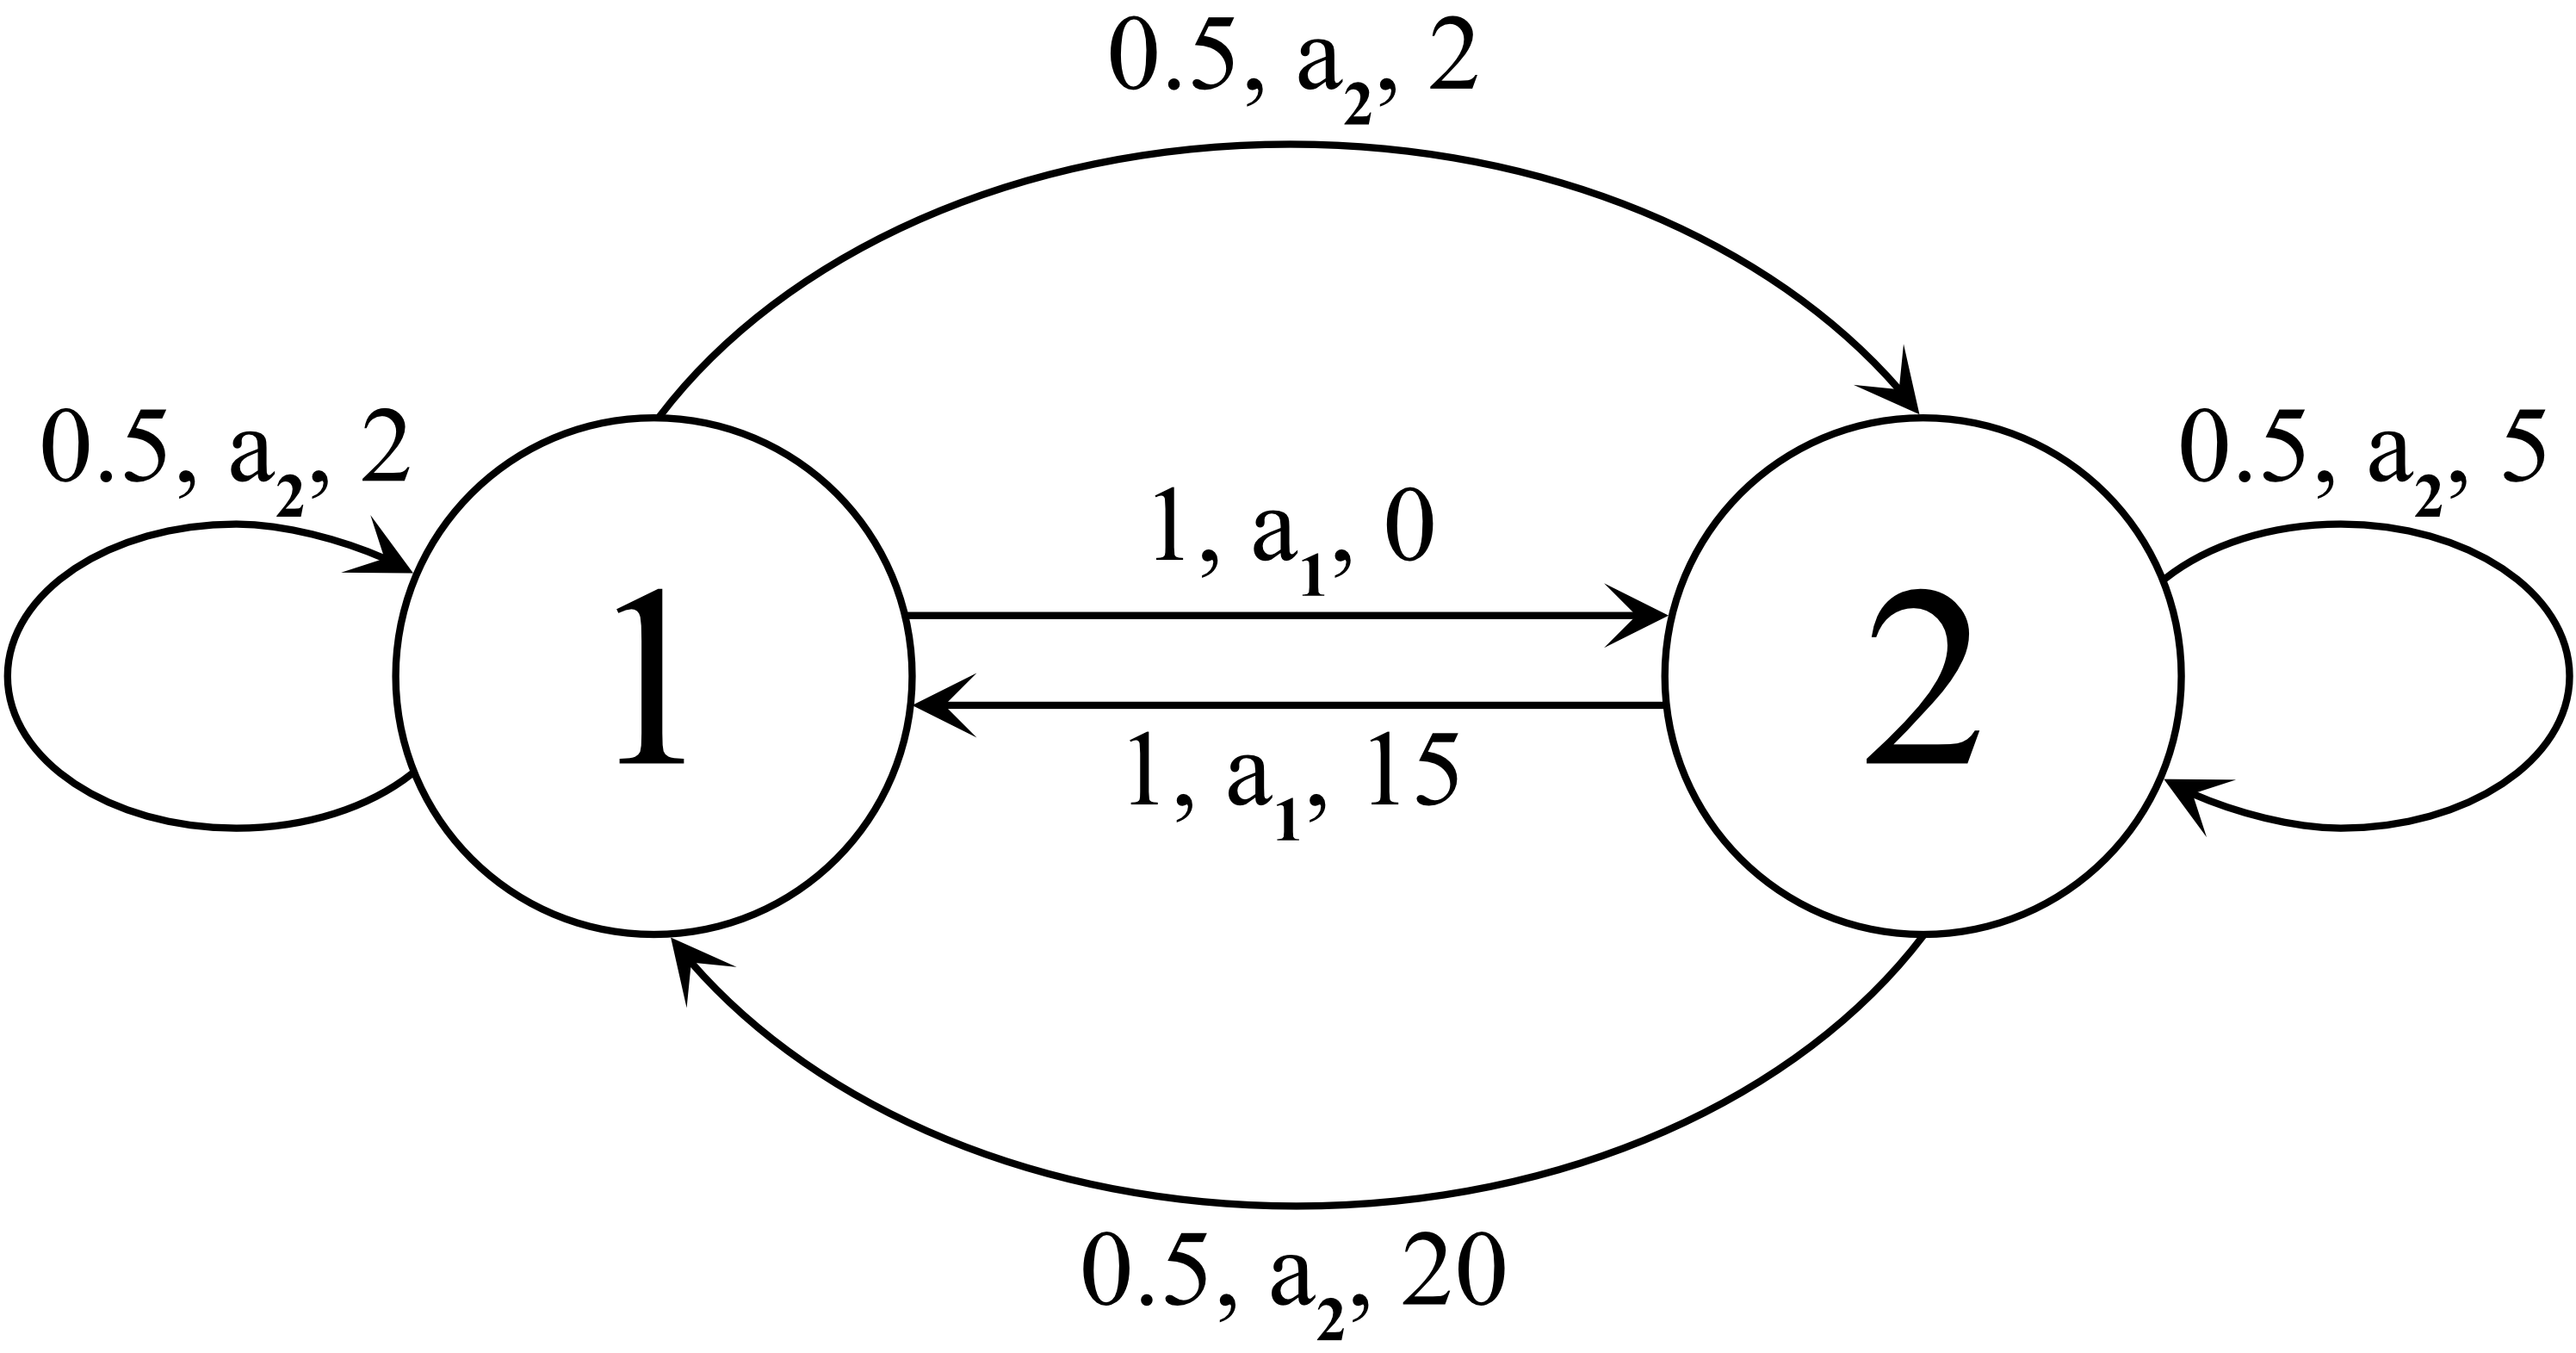
\includegraphics[width=\textwidth]{../thesis/fig/example1.png}
    \caption*{Diagram przejść w modelu dwustanowym}
\end{figure}
\end{column}
\end{columns}
\end{frame}

\begin{frame}{MDP z dwoma stanami -- Wyniki}
\textbf{Weryfikacja poprawności algorytmów:}

\begin{itemize}
    \item Porównanie wyników z obliczeniami analitycznymi
    \item Algorytmy osiągnęły zbieżność do wartości teoretycznych
    \item Błąd aproksymacji poniżej 1\%
\end{itemize}

\vspace{0.5em}
\textbf{Obserwacje:}
\begin{itemize}
    \item \textbf{Niespójność czasowa:} Optymalna reguła pierwszego kroku $\mu^\star$ różni się od optymalnej polityki stacjonarnej $\phi_s^\star$ dla $\alpha < 1$
    \item Decydent zobowiązany osiąga wyższą wartość niż decydent naiwny
    \item Szybka zbieżność (wykładnicza) zgodnie z teorią
\end{itemize}

\vspace{0.5em}
\textbf{Warunki Robbinsa-Monro dla kroków uczenia:}
\[
\eta_n = \frac{\eta_0}{(c + n)^{\kappa}}, \quad
\theta_n = \frac{\theta_0}{(c + n)^{\lambda}}, \quad
\frac{1}{2} < \kappa < \lambda \le 1
\]
\end{frame}

\begin{frame}{Problem zarządzania zapasami}
\textbf{Model:}
\begin{itemize}
    \item Decydent zarządza magazynem z ograniczoną pojemnością
    \item W każdym okresie podejmuje decyzję o zamówieniu
    \item Popyt jest losowy
    \item Koszty: przechowywania, zamówienia, braku zapasu
\end{itemize}

\vspace{0.5em}
\textbf{Parametry środowiska:}
\begin{itemize}
    \item Maksymalna pojemność magazynu: różne konfiguracje
    \item Rozkład popytu: dyskretny, losowy
    \item Dyskontowanie QH: $\alpha = 0.5$, $\beta = 0.9$
\end{itemize}

\vspace{0.5em}
\textbf{Cele eksperymentu:}
\begin{enumerate}
    \item Weryfikacja działania algorytmu w bardziej złożonym środowisku
    \item Analiza zachowania decydenta z uprzedzeniem teraźniejszości
    \item Porównanie z klasycznym podejściem wykładniczym ($\alpha = 1$)
\end{enumerate}
\end{frame}

\begin{frame}{Wyniki eksperymentów -- Zarządzanie zapasami}
\textbf{Kluczowe obserwacje:}

\begin{itemize}
    \item \textbf{Różnica w strategiach:} Decydent QH ($\alpha < 1$) preferuje natychmiastowe nagrody
    \begin{itemize}
        \item Mniejsze zamówienia w pierwszym kroku
        \item Wyższa gotowość akceptacji kosztów braku zapasu
    \end{itemize}
    
    \vspace{0.5em}
    \item \textbf{Zbieżność:} Algorytm QH Q-Learning skutecznie nauczył się polityki
    \begin{itemize}
        \item Stabilizacja wartości Q po odpowiedniej liczbie iteracji
        \item Zgodność z przewidywaniami teoretycznymi
    \end{itemize}
    
    \vspace{0.5em}
    \item \textbf{Porównanie z decydentem wykładniczym:}
    \begin{itemize}
        \item Decydent wykładniczy ($\alpha = 1$) osiąga wyższe wartości długoterminowe
        \item Decydent QH ($\alpha < 1$) maksymalizuje wartość uwzględniając uprzedzenie teraźniejszości
        \item Różne strategie optymalne dla różnych wartości $\alpha$
    \end{itemize}
\end{itemize}
\end{frame}

\begin{frame}{Implementacja i metodologia}
\textbf{Narzędzia i technologie:}
\begin{itemize}
    \item Język: Python 3.8+
    \item Biblioteki: NumPy, SciPy, Matplotlib
    \item Framework testowy: pytest
\end{itemize}

\vspace{0.5em}
\textbf{Struktura kodu:}
\begin{itemize}
    \item \texttt{algorithms/} -- implementacje algorytmów (QH Q-Learning, Policy Evaluation)
    \item \texttt{models/} -- modele środowisk (Inventory, GridWorld)
    \item \texttt{experiments/} -- framework eksperymentalny
    \item \texttt{tests/} -- testy jednostkowe
\end{itemize}

\vspace{0.5em}
\textbf{Walidacja:}
\begin{itemize}
    \item Porównanie z wynikami analitycznymi dla prostych modeli
    \item Testy zbieżności
    \item Weryfikacja własności teoretycznych (kontrakcja, niespójność czasowa)
\end{itemize}
\end{frame}
